\typeout{************************************************}
\typeout{Chapter 8 A ``Tayl'' of Three Remainders}
\typeout{************************************************}
%
\begin{chapterptx}{A ``Tayl'' of Three Remainders}{}{A ``Tayl'' of Three Remainders}{}{}{x:chapter:TaylorSeries}
	%
	%
	\typeout{************************************************}
	\typeout{Section 8.1 The Integral Form of the Remainder}
	\typeout{************************************************}
	%
	\begin{sectionptx}{The Integral Form of the Remainder}{}{The Integral Form of the Remainder}{}{}{x:section:TaylorSeries-IntFormRem}
		Now that we have a rigorous definition of the convergence of a sequence, let's apply this to Taylor series.  Recall that the Taylor series of a function \(f(x)\) expanded about the point \(a\) is given by%
		\begin{equation*}
			\sum_{n=0}^\infty\frac{f^{(n)}(a)}{n!}(x-a)^n=f(a)+\frac{f^{\,\prime}(a)}{1!}(x-a)+\frac{f^{\,\prime\prime}(a)}{2!}(x-a)^2+\cdots
		\end{equation*}
		%
		\par
		When we say that \(f(x)=\sum_{n=0}^\infty\frac{f^{(n)}(a)}{n!}(x-a)^n\) for a particular value of \(x\), what we mean is that the sequence of partial sums%
		\begin{alignat*}{1}
			\amp\left(\sum_{j=0}^n\frac{f^{(j)}(a)}{j!}(x-a)^j\right)_{n=0}^\infty\\
			\amp= \left(f(a), f(a)+\frac{f^{\prime}(a)}{1!}(x-a),f(a)
			+\frac{f^{\prime}(a)}{1!}(x-a)+\frac{f^{\prime\prime}(a)}{2!}(x-a)^2,\ldots\right)
		\end{alignat*}
		converges to the number \(f(x)\). Note that the index in the summation was changed to \(j\) to allow \(n\) to represent the index of the sequence of partial sums. As intimidating as this may look, bear in mind that for a fixed real number \(x\), this is still a sequence of real numbers so, that saying \(f(x)=\sum_{n=0}^\infty\frac{f^{(n)}(a)}{n!}(x-a)^n\) means that \(\lim_{n\rightarrow\infty}\left(\sum_{j=0}^n\frac{f^{(j)}(a)}{j!}(x-a)^j\right)=f(x)\) and in the previous chapter we developed some tools to examine this phenomenon. In particular, we know that \(\lim_{n\rightarrow\infty}\left(\sum_{j=0}^n\frac{f^{(j)}(a)}{j!}(x-a)^j\right)=f(x)\) is equivalent to%
		\begin{equation*}
			\lim_{n\rightarrow\infty}\Biggl[f(x)-\left(\sum_{j=0}^n \frac{f^{(j)}(a)}{j!}(x-a)^j\right)\Biggr]=0\text{.}
		\end{equation*}
		%
		\par
		We have seen an example of this already. \hyperref[x:problem:prob_series-geometric]{Problem~{\xreffont\ref{x:problem:prob_series-geometric}}} of the last chapter basically had you show that  the geometric series, \(1+x+x^2+x^3+\cdots\) converges to \(\frac{1}{1-x}\),for \(|x|\lt 1\) by showing that \(\limit{n}{\infty}{\Biggl[\frac{1}{1-x}-\left(\sum_{j=0}^nx^j\right)\Biggr]=0}\).%
		\par
		There is generally not a readily recognizable closed form for the partial sum for a Taylor series. The geometric series is a special case. Fortunately, for the issue at hand (convergence of a Taylor series), we don't need to analyze the series itself. What we need to show is that the difference between the function and the \(n\)th partial sum converges to zero. This difference is called the \terminology{remainder (of the Taylor series)}. (Why?)%
		\par
		While it is true that the remainder is simply%
		\begin{equation*}
			f(x)-\left(\sum_{j=0}^n\frac{f^{(j)}(a)}{j!}(x-a)^j\right)\text{,}
		\end{equation*}
		this form is not easy to work with. Fortunately, a number of alternate versions of this remainder are available. We will explore these in this chapter.%
		\par
		Recall the result from \hyperref[x:theorem:TaylorsTheorem]{Theorem~{\xreffont\ref{x:theorem:TaylorsTheorem}}} from \hyperref[x:chapter:PowerSeriesQuestions]{Chapter~{\xreffont\ref{x:chapter:PowerSeriesQuestions}}},%
		\begin{align*}
			f(x)=f(a)+\frac{f^{\,\prime}(a)}{1!}(x-a)+\frac{f^{\,\prime\prime}(a)}{2!}(x-a)^2\amp +\cdots+\frac{f^{(n)}(a)}{n!}(x-a)^n\\
			\amp +\frac{1}{n!}\int_{t=a}^xf^{(n+1)}(t)(x-t)^n\dx{ t}\text{.}
		\end{align*}
		%
		\par
		We can use this by rewriting it as%
		\begin{equation*}
			f(x)-\left(\sum_{j=0}^n\frac{f^{(j)}(a)}{j!}(x-a)^j\right)=\frac{1}{n!}\int_{t=a}^xf^{(n+1)}(t)(x-t)^n\dx{ t}\text{.}
		\end{equation*}
		%
		\par
		The expression \(\frac{1}{n!}\int_{t=a}^xf^{(n+1)}(t)(x-t)^n\dx{ t}\) is called the \emph{integral form of the remainder for the Taylor series} of \(f(x)\), and the Taylor series will converge to \(f(x)\) exactly when the sequence \(\lim_{n\rightarrow\infty}\left(\frac{1}{n!}\int_{t=a}^xf^{(n+1)}(t)(x-t)^n\dx{ t}\text{ } \right)\) converges to zero. It turns out that this form of the remainder is often easier to handle than the original \(f(x)-\left(\sum_{j=0}^n\frac{f^{(j)}(a)}{j!}(x-a)^j\right)\) and we can use it to obtain some general results.%
		\begin{theorem}{}{}{x:theorem:thm_TaylorSeries}%
			\terminology{Taylor's series}%
			\par
			\index{series!Taylor's series} If there exists a real number \(B\) such that \(|f^{(n+1)}(t)|\leq B\) for all nonnegative integers \(n\) and for all \(t\) on an interval containing \(a\) and \(x\), then%
			\begin{equation*}
				\lim_{n\rightarrow\infty}\left(\frac{1}{n!}\int_{t=a}^xf^{(n+1)}(t)(x-t)^n\dx{ t}\right)=0
			\end{equation*}
			and so%
			\begin{equation*}
				f(x)=\sum_{n=0}^\infty\frac{f^{(n)}(a)}{n!}(x-a)^n.{}
			\end{equation*}
			%
		\end{theorem}
		In order to prove this, it might help to first prove the following.%
		\begin{lemma}{}{}{x:lemma:lemma_TriangleForIntegral}%
			If \(f\) and \(\abs{f}\) are integrable functions and \(a\leq b\), then%
			\begin{equation*}
				\left|\int_{t=a}^bf(t)\dx{ t}\right|\leq\int_{t=a}^b|f(t)|\dx{ t}. {}
			\end{equation*}
			%
		\end{lemma}
		\begin{problem}{}{g:problem:idp148}%
			\index{Triangle Inequalities!for Integrals} Prove \hyperref[x:lemma:lemma_TriangleForIntegral]{Lemma~{\xreffont\ref{x:lemma:lemma_TriangleForIntegral}}}.%
			\par\smallskip%
			\noindent\textbf{\blocktitlefont Hint}.\hypertarget{g:hint:idp149}{}\quad{}\(-|f(t)|\leq f(t)\leq|f(t)|\).%
		\end{problem}
		\begin{problem}{}{g:problem:idp150}%
			\index{series!Taylor's series!\(f^{(n)}\lt B,\forall\  n\in\NN\imp\) Taylor series converges} Prove \hyperref[x:theorem:thm_TaylorSeries]{Theorem~{\xreffont\ref{x:theorem:thm_TaylorSeries}}}.%
			\par\smallskip%
			\noindent\textbf{\blocktitlefont Hint}.\hypertarget{g:hint:idp151}{}\quad{}You might want to use \hyperref[x:problem:prob_RatioTest]{Problem~{\xreffont\ref{x:problem:prob_RatioTest}}} of \hyperref[x:chapter:Convergence]{Chapter~{\xreffont\ref{x:chapter:Convergence}}}.  Also there are two cases to consider: \(a\lt x\) and \(x\lt a\) (the case \(x=a\) is trivial).  You will find that this is true in general.  This is why we will often indicate that \(t\) is between \(a\) and \(x\) as in the theorem.  In the case \(x\lt a\), notice that%
			\begin{align*}
				\left|\int_{t=a}^xf^{(n+1)}(t)(x-t)^n\dx{ t}\right|\amp =\left|(-1)^{n+1}\int_{t=x}^af^{(n+1)}(t)(t-x)^n\dx{ t}\right|\\
				\amp =\left|\int_{t=x}^af^{(n+1)}(t)(t-x)^n\dx{ t}\right|.
			\end{align*}
			%
		\end{problem}
		\begin{problem}{}{x:problem:prob_Taylor_Series-using}%
			Use \hyperref[x:theorem:thm_TaylorSeries]{Theorem~{\xreffont\ref{x:theorem:thm_TaylorSeries}}} to prove that for any real number \(x\)%
			\begin{enumerate}[font=\bfseries,label=(\alph*),ref=\alph*]
				\item{}\(\displaystyle\sin x=\sum_{n=0}^\infty\frac{(-1)^nx^{2n+1}}{(2n+1)!}\)%
				\item{}\(\displaystyle\cos x= \sum_{n=0}^\infty\frac{(-1)^nx^{2n}}{(2n)!}\)%
				\item\label{x:task:prob_Taylor_Series-using-c}\(\displaystyle e^x=\sum_{n=0}^\infty\frac{x^n}{n!}\)%
			\end{enumerate}
		\end{problem}
		\hyperref[x:task:prob_Taylor_Series-using-c]{Problem~{\xreffont\ref{x:problem:prob_Taylor_Series-using}}.{\xreffont\ref{x:task:prob_Taylor_Series-using-c}}} shows that the Taylor series of \(e^x\) expanded at zero converges to \(e^x\) for any real number \(x\). \hyperref[x:theorem:thm_TaylorSeries]{Theorem~{\xreffont\ref{x:theorem:thm_TaylorSeries}}} can be used in a similar fashion to show that%
		\begin{equation*}
			e^x=\sum_{n=0}^\infty\frac{e^a(x-a)^n}{n!}
		\end{equation*}
		for any real numbers \(a\) and \(x\).%
		\par
		Recall that \hyperref[x:chapter:CalcIn17th18thCentury]{Chapter~{\xreffont\ref{x:chapter:CalcIn17th18thCentury}}} we showed that if we define the function \(E(x)\) by the power series \(\sum_{n=0}^\infty\frac{x^n}{n!}\) then \(E(x+y)=E(x)E(y)\). This, of course, is just the familiar addition property of integer exponents extended to any real number. In \hyperref[x:chapter:CalcIn17th18thCentury]{Chapter~{\xreffont\ref{x:chapter:CalcIn17th18thCentury}}} we had to \emph{assume} that defining \(E(x)\) as a series was meaningful because we did not address the convergence of the series in that chapter. Now that we know the series converges for any real number we see that the definition%
		\begin{equation*}
			f(x) = e^x = \sum_{n=0}^\infty\frac{x^n}{n!}
		\end{equation*}
		is in fact valid.%
		\par
		Assuming that we can differentiate this series term-by-term it is straightforward to show that \(f^\prime(x) = f(x)\).%
		\begin{aside}{}{g:aside:idp152}%
			We can, but that proof will have to wait for a few more chapters.%
		\end{aside}
		Along with Taylor's formula this can then be used to show that \(e^{a+b}=e^ae^b\) more elegantly than the rather cumbersome proof in \hyperref[x:mrow:eq_ExponentAdditionProperty]{equation~({\xreffont\ref{x:mrow:eq_ExponentAdditionProperty}})}, as the following problem shows.%
		\begin{problem}{}{g:problem:idp153}%
			\index{\(e^x\)!\(e^{a+b}=e^ae^b\)} Recall that if \(f(x)=e^x\) then \(f^\prime(x) = e^x\). Use this along with the Taylor series expansion of \(e^x\) about \(a\) to show that%
			\begin{equation*}
				e^{a+b}=e^ae^b.
			\end{equation*}
			%
		\end{problem}
		\hyperref[x:theorem:thm_TaylorSeries]{Theorem~{\xreffont\ref{x:theorem:thm_TaylorSeries}}} is a nice ``first step'' toward a rigorous theory of the convergence of Taylor series, but it is not applicable in all cases. For example, consider the function \(f(x)=\sqrt{1+x}\). As we saw in \hyperref[x:chapter:CalcIn17th18thCentury]{Chapter~{\xreffont\ref{x:chapter:CalcIn17th18thCentury}}}, \hyperref[x:problem:prob_SqrtSeriesProb]{Problem~{\xreffont\ref{x:problem:prob_SqrtSeriesProb}}}, this function's Maclaurin series (the binomial series for \(\left(1+x\right)^{1/2})\)appears to be converging to the function for \(x\in(-1,1)\). While this is, in fact, true, the above proposition does not apply. If we consider the derivatives of \(f(t)=(1+t)^{1/2}\), we obtain:%
		\begin{align*}
			f^\prime(t)\amp =\frac{1}{2}(1+t)^{\frac{1}{2}-1}\\
			f^{\prime\prime}(t)\amp =\frac{1}{2}\left(\frac{1}{2}-1\right)(1+t)^{\frac{1}{2}-2}\\
			f^{\prime\prime\prime}(t)\amp =\frac{1}{2}\left(\frac{1}{2}-1\right)\left(\frac{1}{2}-2 \right)(1+t)^{\frac{1}{2}-3}\\
			\amp \vdots\\
			f^{(n+1)}(t)\amp =\frac{1}{2}\left(\frac{1}{2}-1\right)\left(\frac{1}{2}-2\right) \cdots\left(\frac{1}{2}-n\right)(1+t)^{\frac{1}{2}-(n+1)}\text{.}
		\end{align*}
		%
		\par
		Notice that%
		\begin{equation*}
			\left|f^{(n+1)}(0)\right|=\frac{1}{2}\left(1-\frac{1}{2}\right)\left(2-\frac{1}{2}\right)\cdots\left(n-\frac{1}{2}\right)\text{.}
		\end{equation*}
		%
		\par
		Since this sequence grows without bound as \(n\rightarrow\infty\), then there is no chance for us to find a number \(B\) to act as a bound for all of the derviatives of \(f\) on any interval containing 0 and\(\) \(x\), and so the hypothesis of \hyperref[x:theorem:thm_TaylorSeries]{Theorem~{\xreffont\ref{x:theorem:thm_TaylorSeries}}} will never be satisfied. We need a more delicate argument to prove that%
		\begin{equation*}
			\sqrt{1+x}=1+\frac{1}{2}x+\frac{\frac{1}{2}\left(\frac{1}{2}-1\right)}{2!}x^2+\frac{\frac{1}{2}\left(\frac{1}{2}-1\right)\left(\frac{1}{2}-2\right)}{3!}x^3+\cdots
		\end{equation*}
		is valid for \(x\in(-1,1)\). To accomplish this task, we will need to express the remainder of the Taylor series differently. Fortunately, there are at least two such alternate forms.%
	\end{sectionptx}
	%
	%
	\typeout{************************************************}
	\typeout{Section 8.2 Lagrange's Form of the Remainder}
	\typeout{************************************************}
	%
	\begin{sectionptx}{Lagrange's Form of the Remainder}{}{Lagrange's Form of the Remainder}{}{}{x:section:TaylorSeries-LagrFormRem}
		Joseph-Louis Lagrange \index{Lagrange, Joseph-Louis} provided an alternate form for the remainder in Taylor series in his 1797 work \textbraceleft{}Th\textbackslash{}a'eorie des functions analytiques.\textbraceright{} Lagrange's form of the remainder is as follows.%
		\begin{theorem}{}{}{x:theorem:thm_LagrangeRemainder}%
			\terminology{Lagrange's Form of the Remainder}%
			\par
			\index{Lagrange's form of the remainder} Suppose \(f\) is a function such that \(f^{(n+1)}(t)\) is continuous on an interval containing \(a\) and \(x\). Then%
			\begin{equation*}
				f(x)-\left(\sum_{j=0}^n\frac{f^{(j)}(a)}{j!}(x-a)^j\right)=\frac{f^{\, (n+1)}(c)}{(n+1)!}(x-a)^{n+1}
			\end{equation*}
			where \(c\) is some number between \(a\) and \(x\).%
		\end{theorem}
		\begin{proof}{}{g:proof:idp154}
			Note first that the result is true when \(x=a\) as both sides reduce to 0 (in that case \(c=x=a\).) We will prove the case where \(a\lt x\); the case \(x\lt a\) will be an exercise.%
			\par
			First, we already have%
			\begin{equation*}
				f(x)-\left(\sum_{j=0}^n\frac{f^{(j)}(a)}{j!}(x-a)^j\right)=\frac{1}{n!} \int_{t=a}^xf^{(n+1)}(t)(x-t)^n\dx{ t}
			\end{equation*}
			so it suffices to show that%
			\begin{equation*}
				\int_{t=a}^xf^{(n+1)}(t)(x-t)^n\dx{ t}=\,\frac{f^{\,(n+1)}(c)}{n+1}(x-a)^{n+1}
			\end{equation*}
			for some \(c\) with \(c\in[\,a,x]\). To this end, let%
			\begin{equation*}
				M=\max_{a\le t\le x}\left(f^{(n+1)}(t)\right)
			\end{equation*}
			and%
			\begin{equation*}
				m=\min_{a\le t\le x}\left(f^{(n+1)}(t)\right)\text{.}
			\end{equation*}
			%
			\par
			Note that for all \(t\in[\,a,x]\), we have \(m\leq f^{(n+1)}(t)\leq M\). Since \(x-t\geq 0\), this gives us%
			\begin{equation}
				m\left(x-t\right)^n\leq f^{(n+1)}(t)(x-t)^n\leq M(x-t)^n\label{x:men:eq_LagRem1}
			\end{equation}
			and so%
			\begin{equation}
				\int_{t=a}^xm\left(x-t\right)^n\dx{ t}\leq\int_{t=a}^xf^{(n+1)}(t)(x-t)^n\dx{ t}\leq \int_{t=a}^xM(x-t)^n\dx{ t}\text{.}\label{x:men:eq_LagRem2}
			\end{equation}
			%
			\par
			Computing the outside integrals, we have%
			\begin{equation*}
				m\int_{t=a}^x\left(x-t\right)^n\dx{ t}\leq\int_{t=a}^xf^{(n+1)}(t)(x-t)^n\dx{ t}\leq M\int_{t=a}^x(x-t)^n\dx{ t}
			\end{equation*}
			%
			\begin{equation}
				m\frac{(x-a)^{n+1}}{n+1}\leq\int_{t=a}^xf^{(n+1)}(t)(x-t)^n\dx{ t}\leq M\frac{(x-a)^{n+1}}{n+1}\label{x:men:eq_LagRem3}
			\end{equation}
			%
			\begin{equation*}
				m\leq\frac{\int_{t=a}^xf^{(n+1)}(t)(x-t)^n\dx{ t}}{\left(\frac{(x-a)^{n+1}}{n+1} \right)}\leq M\text{.}
			\end{equation*}
			%
			\par
			Since%
			\begin{equation*}
				\frac{\int_{t=a}^xf^{(n+1)}(t)(x-t)^n\dx{ t}}{\left(\frac{(x-a)^{n+1}}{n+1} \right)}
			\end{equation*}
			is a value that lies between the maximum and minimum of \(f^{(n+1)}\) on \([\,a,x]\), then by the Intermediate Value Theorem, there must exist a number \(c\in[\,a,x]\) with%
			\begin{equation*}
				f^{(n+1)}(c)=\frac{\int_{t=a}^xf^{(n+1)}(t)(x-t)^n\dx{ t}}{\left( \frac{(x-a)^{n+1}}{n+1}\right)}\text{.}
			\end{equation*}
			%
			\par
			This gives us%
			\begin{equation*}
				\int_{t=a}^xf^{(n+1)}(t)(x-t)^n\dx{ t}=\,\frac{f^{\,(n+1)}(c)}{n+1}(x-a)^{n+1}\text{.}
			\end{equation*}
			%
			\par
			And the result follows.%
		\end{proof}
		\begin{problem}{}{g:problem:idp155}%
			\index{Lagrange's form of the remainder!\(x\lt a\)} Prove \hyperref[x:theorem:thm_LagrangeRemainder]{Theorem~{\xreffont\ref{x:theorem:thm_LagrangeRemainder}}} for the case where \(x\lt a\).%
			\par\smallskip%
			\noindent\textbf{\blocktitlefont Hint}.\hypertarget{g:hint:idp156}{}\quad{}Note that%
			\begin{equation*}
				\int_{t=a}^xf^{(n+1)}(t)(x-t)^n\dx{ t}=(-1)^{n+1}\int_{t=x}^af^{(n+1)}(t)(t-x)^n\dx{ t}\text{.}
			\end{equation*}
			%
			\par
			Use the same argument on this integral.  It will work out in the end.  Really!  You just need to keep track of \emph{all} of the negatives.%
		\end{problem}
		This is \emph{not} Lagrange's proof.  He did not use the integral form of the remainder.  However, this is similar to Lagrange's proof in that he also used the Intermediate Value Theorem (IVT) \index{Intermediate Value Theorem (IVT)} and Extreme Value Theorem (EVT) \index{Extreme Value Theorem (EVT)} much as we did.  In Lagrange's day, these were taken to be obviously true for a continuous function and we have followed Lagrange's \index{Lagrange, Joseph-Louis} lead by assuming the IVT and the EVT. However, in mathematics we need to keep our assumptions few and simple.  The IVT and the EVT do not satisfy this need in the sense that both can be proved from simpler ideas.  We will return to this in \hyperref[x:chapter:IVTandEVT]{Chapter~{\xreffont\ref{x:chapter:IVTandEVT}}}.%
		\par
		Also, a word of caution about this: Lagrange's form of the remainder is \(\frac{f^{\,(n+1)}(c)}{(n+1)!}\) \((x-a)^{n+1}\), where \(c\) is some number between \(a\) and \(x\).  The proof does not indicate what this \(c\) might be and, in fact, this \(c\) changes as \(n\) changes. All we know is that this \(c\) lies between \(a\) and \(x\).  To illustrate this issue and its potential dangers, consider the following problem where we have a chance to compute the value of \(c\) for the function \(f(x)=\frac{1}{1+x}\).%
		\begin{problem}{}{g:problem:idp157}%
			This problem investigates the Taylor series representation%
			\begin{equation*}
				\frac{1}{1+x}=1-x+x^2-x^3+\cdots\text{.}
			\end{equation*}
			%
			\begin{enumerate}[font=\bfseries,label=(\alph*),ref=\alph*]
				\item{}Use the fact that \(\frac{1-(-x)^{n+1}}{1+x}=1-x+x^2-x^3+\cdots+(-x)^n\) to compute the remainder \(\frac{1}{1+x}-\left(1-x+x^2-x^3+\cdots+(-x)^n\right)\). Specifically, compute this remainder when \(x=1\) and conclude that the Taylor series does not converge to \(\frac{1}{1+x}\) when \(x=1\).%
				\item{}Compare the remainder in part a with the Lagrange form of the remainder to determine what \(c\) is when \(x=1\).%
				\item{}Consider the following argument: If \(f(x)=\frac{1}{1+x}\), then%
				\begin{equation*}
					f^{(n+1)}(c)=\frac{(-1)^{n+1}(n+1)!}{(1+c)^{n+2}}
				\end{equation*}
				so the Lagrange form of the remainder when \(x=1\) is given by%
				\begin{equation*}
					\frac{(-1)^{n+1}(n+1)!}{(n+1)!(1+c)^{n+2}}=\frac{(-1)^{n+1}}{(1+c)^{n+2}}
				\end{equation*}
				where \(c\in[\,0,1]\).  It can be seen in part b that \(c\neq 0\).  Thus \(1+c>1\) and so by \hyperref[x:problem:prob_sequences3]{Problem~{\xreffont\ref{x:problem:prob_sequences3}}} of \hyperref[x:chapter:Convergence]{Chapter~{\xreffont\ref{x:chapter:Convergence}}}, the Lagrange remainder converges to \(0\) as \(n\rightarrow\infty\).  This argument would suggest that the Taylor series converges to \(\frac{1}{1+x}\) for \(x=1\).  However, we know from part (a) that this is incorrect.  What is wrong with the argument?%
			\end{enumerate}
		\end{problem}
		Even though there are potential dangers in misusing the Lagrange form of the remainder, it is a useful form.  For example, armed with the Lagrange form of the remainder, we can prove the following theorem.%
		\begin{theorem}{}{}{x:theorem:thm_BinomialSeriesConverges}%
			\index{series!Binomial Series, the}%
			\index{Binomial Series, the!converges on the interval \([0,1]\)}%
			The binomial series%
			\begin{equation*}
				1+\frac{1}{2}x+\frac{\frac{1}{2}\left(\frac{1}{2}-1\right)}{2!}x^2+\frac{\frac{1}{2}\left(\frac{1}{2}-1\right)\left(\frac{1}{2}-2\right)}{3!}x^3+\cdots
			\end{equation*}
			converges to \(\sqrt{1+x}\) for \(x\in[0,1]\).%
		\end{theorem}
		\begin{proof}{}{g:proof:idp158}
			First note that the binomial series is, in fact, the Taylor series for the function \(f(x)=\sqrt{1+x}\) expanded about \(a=0\). If we let \(x\) be a fixed number with \(0\leq x\leq 1\), then it suffices to show that the Lagrange form of the remainder converges to \(0\). With this in mind, notice that%
			\begin{equation*}
				f^{(n+1)}(t)=\left(\frac{1}{2}\right)\left(\frac{1}{2}-1\right)\cdots\left(\frac{1}{2}-n\right)\left(1+t\right)^{\frac{1}{2}-(n+1)}
			\end{equation*}
			and so the Lagrange form of the remainder is%
			\begin{equation*}
				\frac{f^{(n+1)}(c)}{(n+1)!}x^{n+1}= \frac{\left(\frac{1}{2}\right)\left(\frac{1}{2}-1\right)\cdots \left(\frac{1}{2}-n\right)}{(n+1)!}\frac{x^{n+1}}{(1+c)^{n+\frac{1}{2}}}
			\end{equation*}
			where \(c\) is some number between \(0\) and \(x\). Since \(0\leq x\leq 1\) and \(1+c\geq 1\), then we have \(\frac{1}{1+c}\leq 1\), and so%
			\begin{align*}
				0\amp \leq \left|\frac{\left(\frac{1}{2}\right)\left(\frac{1}{2}-1\right)\cdots\left(\frac{1}{2}-n\right)}{(n+1)!}\frac{x^{n+1}}{(1+c)^{n+\frac{1}{2}}}\right|\\
				\amp =\frac{\left(\frac{1}{2}\right)\left(1-\frac{1}{2}\right)\cdots\left(n-\frac{1}{2}\right)}{(n+1)!}\frac{x^{n+1}}{(1+c)^{n+\frac{1}{2}}}\\
				\amp =\frac{\left(\frac{1}{2}\right)\left(\frac{1}{2}\right)\left(\frac{3}{2}\right)\left(\frac{5}{2}\right)\cdots\left(\frac{2n-1}{2}\right)}{(n+1)!}\left(x^{n+1}\right)\frac{1}{(1+c)^{n+\frac{1}{2}}}\\
				\amp \leq\frac{1\cdot 1\cdot 3\cdot5\cdot\,\cdots\,\cdot\left(2n-1\right)}{2^{^{n+1}}(n+1)!}\\
				\amp =\frac{1\cdot 3\cdot 5\cdot\,\cdots\,\cdot\left(2n-1\right)\cdot 1}{2\cdot4\cdot 6\cdot\,\cdots\,\cdot 2n\cdot\left(2n+2\right)}\\
				\amp =\frac{1}{2}\cdot\frac{3}{4}\cdot\frac{5}{6}\cdot\cdots\,\cdot\frac{2n-1}{2n}\cdot\frac{1}{2n+2}\\
				\amp \leq\frac{1}{2n+2}\text{.}
			\end{align*}
			%
			\par
			Since \(\lim_{n\rightarrow\infty}\frac{1}{2n+2}=0=\,\lim_{n\rightarrow\infty}0\), then by the Squeeze Theorem,%
			\begin{equation*}
				\lim_{n\rightarrow\infty}\abs{\frac{f^{(n+1)}(c)}{(n+1)!}x^{n+1}}=0, \text{ so } \lim_{n\rightarrow\infty}\left(\frac{f^{(n+1)}(c)}{(n+1)!}x^{n+1}\right)=0\text{.}
			\end{equation*}
			%
			\par
			Thus the Taylor series%
			\begin{equation*}
				1+\frac{1}{2}x+\frac{\frac{1}{2}\left(\frac{1}{2}-1\right)}{2!}x^2+\frac{\frac{1}{2}\left(\frac{1}{2}-1\right)\left(\frac{1}{2}-2\right)}{3!}x^3+\cdots
			\end{equation*}
			converges to \(\sqrt{1+x}\) for \(0\leq x\leq 1\).%
		\end{proof}
		Unfortunately, this proof will not work for \(-1\lt x\lt 0\). In this case, the fact that \(x\leq c\leq 0\) makes\(\,1+c\leq 1\). Thus \(\frac{1}{1+c}\geq 1\) and so the inequality%
		\begin{equation*}
			\frac{\left(\frac{1}{2}\right)\left(\frac{1}{2}\right)\left(\frac{3}{2}\right)\left(\frac{5}{2}\right)\cdots\left(\frac{2n-1}{2}\right)}{(n+1)!}\frac{|x|^{n+1}}{(1+c)^{n+\frac{1}{2}}}\leq\frac{1\cdot 1\cdot 3\cdot 5\cdot\,\cdots\,\cdot\left(2n-1\right)}{2^{^{n+1}}(n+1)!}
		\end{equation*}
		may not hold.%
		\begin{problem}{}{x:problem:prob_Taylor_Series-Binomial_Series_and}%
			\index{series!Binomial Series, the!Binomial Series is a Taylor series} Show that if \(-\frac{1}{2}\leq x\leq c\leq 0\), then \(|\frac{x}{1+c}|\leq 1\) and modify the above proof to show that the binomial series converges to \(\sqrt{1+x}\) for \(x\in\left[-\frac{1}{2},0\right]\).%
		\end{problem}
		To take care of the case where \(-1\lt x\lt -\frac{1}{2}\), we will use yet another form of the remainder for Taylor series. However before we tackle that, we will use the Lagrange form of the remainder to address something mentioned in \hyperref[x:chapter:PowerSeriesQuestions]{Chapter~{\xreffont\ref{x:chapter:PowerSeriesQuestions}}}. Recall that we noticed that the series representation%
		\begin{equation*}
			\frac{1}{1+x}=1-x+x^2-x^3+\cdots
		\end{equation*}
		did not work when \(x=1\), however we noticed that the series obtained by integrating term by term did seem to converge to the antiderivative of \(\frac{1}{1+x}\). Specifically, we have the Taylor series%
		\begin{equation*}
			\ln\left(1+x\right)=x-\frac{1}{2}x^2+\frac{1}{3}x^3-\cdots\text{.}
		\end{equation*}
		%
		\par
		Substituting \(x=1\) into this provided the convergent series \(1-\frac{1}{2}+\frac{1}{3}-\frac{1}{4}+\cdots\). We made the claim that this, in fact, converges to \(\ln 2\), but that this was not obvious. The Lagrange form of the remainder gives us the machinery to prove this.%
		\begin{problem}{}{g:problem:idp159}%
			\begin{enumerate}[font=\bfseries,label=(\alph*),ref=\alph*]
				\item{}Compute the Lagrange form of the remainder for the Maclaurin series for \(\ln\left(1+x\right)\).%
				\item{}Show that when \(x=1\), the Lagrange form of the remainder converges to \(0\) and so the equation \(\ln 2=1-\frac{1}{2}+\frac{1}{3}-\frac{1}{4}+\cdots\) is actually correct.%
			\end{enumerate}
		\end{problem}
	\end{sectionptx}
	%
	%
	\typeout{************************************************}
	\typeout{Section 8.3 Cauchy's Form of the Remainder}
	\typeout{************************************************}
	%
	\begin{sectionptx}{Cauchy's Form of the Remainder}{}{Cauchy's Form of the Remainder}{}{}{x:section:TaylorSeries-CauchyFormRem}
		In his 1823 work, \textit{Résumée des leçons données á l'ecole royale polytechnique sur le calcul infintésimal,} Augustin Cauchy \index{Cauchy, Augustin} provided another form of the remainder for Taylor series.%
		\begin{theorem}{}{}{x:theorem:thm_CauchyRemainder}%
			\terminology{Cauchy's Form of the Remainder}%
			\par
			\index{sequences!Cauchy sequences!Cauchy's remainder} Suppose \(f\) is a function such that \(f^{(n+1)}(t)\) is continuous on an interval containing \(a\) and \(x\). Then%
			\begin{equation*}
				f(x)-\left(\sum_{j=0}^n\frac{f^{(j)}(a)}{j!}(x-a)^j\right)=\frac{f^{\, (n+1)}(c)}{n!}(x-c)^n(x-a)
			\end{equation*}
			where \(c\) is some number between \(a\) and \(x\).%
		\end{theorem}
		\begin{problem}{}{g:problem:idp160}%
			\index{series!Taylor's series!Cauchy Remainder} Prove \hyperref[x:theorem:thm_CauchyRemainder]{Theorem~{\xreffont\ref{x:theorem:thm_CauchyRemainder}}} using an argument similar to the one used in the proof of \hyperref[x:theorem:thm_LagrangeRemainder]{Theorem~{\xreffont\ref{x:theorem:thm_LagrangeRemainder}}}. Don't forget there are two cases to consider.%
		\end{problem}
		Using Cauchy's form of the remainder, we can prove that the binomial series%
		\begin{equation*}
			1+\frac{1}{2}x+\frac{\frac{1}{2}\left(\frac{1}{2}-1\right)}{2!}x^2+\frac{\frac{1}{2}\left(\frac{1}{2}-1\right)\left(\frac{1}{2}-2\right)}{3!}x^3+\cdots
		\end{equation*}
		converges to \(\sqrt{1+x}\) for \(x\in(-1,0).\)%
		\begin{aside}{}{g:aside:idp161}%
			Strictly speaking we only need to show this for \(x\in(-1,-1/2).\)In \hyperref[x:problem:prob_Taylor_Series-Binomial_Series_and]{problem~{\xreffont\ref{x:problem:prob_Taylor_Series-Binomial_Series_and}}} we covered\(x\in (-1/2,0)\).%
		\end{aside}
		With this in mind, let \(x\) be a fixed number with \(-1\lt x\lt 0\) and consider that the binomial series is the Maclaurin series for the function \(f(x)=(1+x)^{\frac{1}{2}}\). As we saw before,%
		\begin{equation*}
			f^{(n+1)}(t)=\left(\frac{1}{2}\right)\left(\frac{1}{2}-1\right)\cdots\left(\frac{1}{2}-n\right)\left(1+t\right)^{\frac{1}{2}-(n+1)}\text{,}
		\end{equation*}
		so the Cauchy form of the remainder is given by%
		\begin{equation*}
			0\le\abs{\frac{f^{(n+1)}(c)}{n!}(x-c)^n(x-0)}= \abs{\frac{\left(\frac{1}{2}\right)\left(\frac{1}{2}-1\right)\cdots\left(\frac{1}{2}-n\right)}{n!}\frac{(x-c)^n}{(1+c)^{n+\frac{1}{2}}}\cdot x}
		\end{equation*}
		where \(c\) is some number with \(x\leq c\leq 0\). Thus we have%
		\begin{align*}
			0\amp \leq\left|\frac{\left(\frac{1}{2}\right)\left(\frac{1}{2}-1\right)\cdots\left(\frac{1}{2}-n\right)}{n!}\frac{(x-c)^nx}{(1+c)^{n+\frac{1}{2}}}\right|\\
			\amp =\frac{\left(\frac{1}{2}\right)\left(1-\frac{1}{2}\right)\cdots\left(n-\frac{1}{2}\right)}{n!}\frac{|x-c|^n|x|}{(1+c)^{n+\frac{1}{2}}}\\
			\amp =\frac{\left(\frac{1}{2}\right)\left(\frac{1}{2}\right)\left(\frac{3}{2}\right)\left(\frac{5}{2}\right)\cdots\left(\frac{2n-1}{2}\right)}{n!}\frac{(c-x)^n}{(1+c)^n}\frac{|\,x|}{\sqrt{1+c}}\\
			\amp =\frac{1\cdot 1\cdot 3\cdot 5\cdot\,\cdots\,\cdot\left(2n-1\right)}{2^{^{n+1}}n!}\left(\frac{c-x}{1+c}\right)^n\frac{|\,x|}{\sqrt{1+c}}\\
			\amp =\frac{1\cdot 1\cdot 3\cdot 5\cdot\,\cdots\,\cdot\left(2n-1\right)}{2\cdot 2\cdot 4\cdot 6\cdot\,\cdots\,\cdot 2n}\left(\frac{c-x}{1+c}\right)^n\frac{|\,x|}{\sqrt{1+c}}\\
			\amp =\frac{1}{2}\cdot\frac{1}{2}\cdot\frac{3}{4}\cdot\frac{5}{6}\cdot\cdots\,\cdot\frac{2n-1}{2n}\cdot\left(\frac{c-x}{1+c}\right)^n\frac{|\,x|}{\sqrt{1+c}}\\
			\amp \leq\left(\frac{c-x}{1+c}\right)^n\frac{|\,x|}{\sqrt{1+c}}\text{.}
		\end{align*}
		%
		\par
		Notice that if \(-1\lt x\leq c\),\(\) then \(0\lt 1+x\leq 1+c\). Thus \(0\lt \frac{1}{1+c}\leq\frac{1}{1+x}\) and \(\frac{1}{\sqrt{1+c}}\leq\frac{1}{\sqrt{1+x}}\). Thus we have%
		\begin{equation*}
			0\leq\left|\frac{\left(\frac{1}{2}\right)\left(\frac{1}{2}-1\right)\cdots\left(\frac{1}{2}-n\right)}{n!}\frac{(x-c)^nx}{(1+c)^{n+\frac{1}{2}}}\right|\leq\left(\frac{c-x}{1+c}\right)^n\frac{|\,x|}{\sqrt{1+x}}\text{.}
		\end{equation*}
		%
		\begin{problem}{}{g:problem:idp162}%
			\index{Binomial Series, the!\(g(c)=\frac{c-x}{1+c}\) is increasing}\index{\(g(c)=\frac{c-x}{1+c}\) is increasing on \([x,0]\)} Suppose \(-1\lt x\leq c\leq 0\) and consider the function \(g(c)=\frac{c-x}{1+c}\). Show that on \([x,0]\), \(g\) is increasing and use this to conclude that for \(-1\lt x\leq c\leq 0\),%
			\begin{equation*}
				\frac{c-x}{1+c}\leq|x|\text{.}
			\end{equation*}
			%
			\par
			Use this fact to finish the proof that the binomial series converges to \(\sqrt{1+x}\) for \(-1\lt x\lt 0\).%
		\end{problem}
		The proofs of both the Lagrange form and the Cauchy form of the remainder for Taylor series made use of two crucial facts about continuous functions. First, we assumed the Extreme Value Theorem: Any continuous function on a closed%
		\begin{figureptx}{\href{https://mathshistory.st-andrews.ac.uk/Biographies/Cauchy/}{Augustin Cauchy}\protect\footnotemark{}}{g:figure:idp163}{}%
			\index{Cauchy, Augustin!portrait of}%
			\begin{image}{0.36}{0.28}{0.36}%
				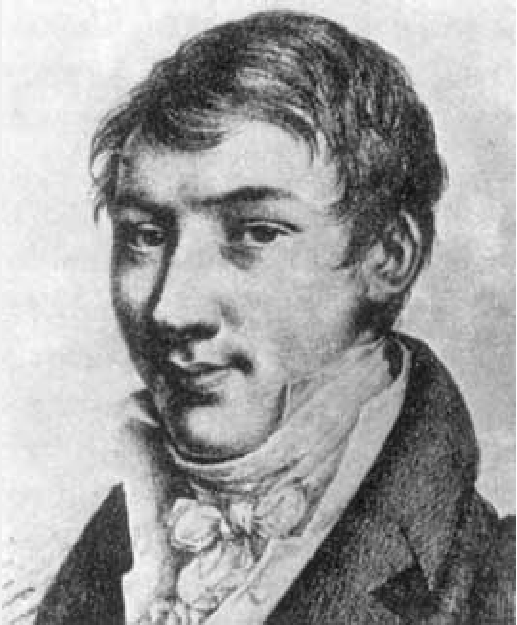
\includegraphics[width=\linewidth]{external/images/Cauchy.png}
			\end{image}%
			\tcblower
		\end{figureptx}%
		\footnotetext[14]{\nolinkurl{mathshistory.st-andrews.ac.uk/Biographies/Cauchy/}\label{g:fn:idp164}}%
		bounded interval assumes its maximum and minimum somewhere on the interval. Second, we assumed that any continuous function satisfied the Intermediate Value Theorem: If a continuous function takes on two different values, then it must take on any value between those two values.%
		\par
		Mathematicians in the late \(1700\)s and early \(1800\)s typically considered these facts to be intuitively obvious.  This was natural since our understanding of continuity at that time was, solely, intuitive.  Intuition is a useful tool, but as we have seen before it is also unreliable.  For example consider the following function.%
		\begin{align}
			f(x)= 
			\begin{cases}
				x\sin\left(\frac{1}{x}\right),\amp \text{if } x\neq 0,\\
				0, \amp \text{ if } x=0 
			\end{cases} \text{.}\label{x:mrow:xsin1x}
		\end{align}
		%
		\par
		Is this function continuous at 0?  Near zero its graph looks like this:%
		\begin{figureptx}{\hyperref[x:mrow:xsin1x]{Formula~({\xreffont\ref{x:mrow:xsin1x}})} near \(0\).}{g:figure:idp165}{}%
			\begin{image}{0}{1}{0}%
				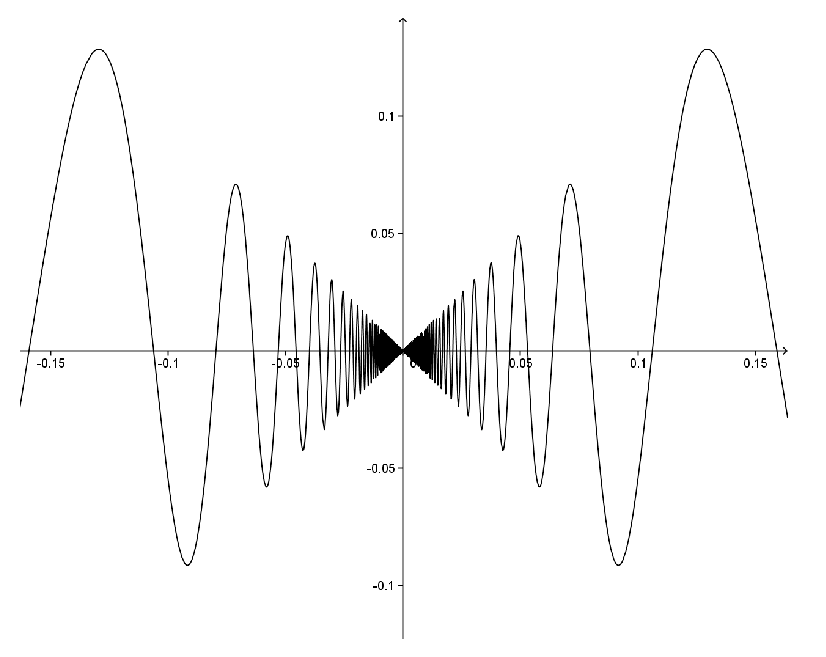
\includegraphics[width=\linewidth]{external/images/Ch5fig4.png}
			\end{image}%
			\tcblower
		\end{figureptx}%
		but this graph must be taken with a grain of salt as \(\sin
		\left(\frac{1}{x}\right)\) oscillates infinitely often as \(x\) nears zero.%
		\par
		No matter what your guess may be, it is clear that it is hard to analyze such a function armed with only an intuitive notion of continuity.  We will revisit this example in the next chapter.%
		\par
		As with convergence, continuity is more subtle than it first appears.%
		\par
		We put convergence on solid ground by providing a completely analytic definition in the previous chapter.  What we need to do in the next chapter is provide a completely rigorous definition for continuity.%
	\end{sectionptx}
	%
	%
	\typeout{************************************************}
	\typeout{Section 8.4 Additional Problems}
	\typeout{************************************************}
	%
	\begin{sectionptx}{Additional Problems}{}{Additional Problems}{}{}{x:section:TaylorSeries-AddProb}
		\begin{problem}{}{g:problem:idp166}%
			Find the Integral form, Lagrange form, and Cauchy form of the remainder for Taylor series for the following functions expanded about the given values of \(\,a\).%
			\begin{enumerate}[font=\bfseries,label=(\alph*),ref=\alph*]
				\item{}\(f(x)=e^x\), \(a=0\)%
				\item{}\(f(x)=\sqrt{x}\), \(a=1\)%
				\item{}\(f(x)=(1+x)^\alpha\), \(a=0\)%
				\item{}\(f(x)=\frac{1}{x}\), \(a=3\)%
				\item{}\(f(x)=\ln x,\ a=2\)%
				\item{}\(f(x)=\cos x, a=\frac{\pi}{2}\)%
			\end{enumerate}
		\end{problem}
	\end{sectionptx}
\end{chapterptx}
%
%